%%%%%%%%%%%%%%%%%%%%%%%%%%%%%%%%%%%%%%%%%
% fphw Assignment
% LaTeX Template
% Version 1.0 (27/04/2019)
%
% This template originates from:
% https://www.LaTeXTemplates.com
%
% Authors:
% Class by Felipe Portales-Oliva (f.portales.oliva@gmail.com) with template 
% content and modifications by Vel (vel@LaTeXTemplates.com)
%
% Template (this file) License:
% CC BY-NC-SA 3.0 (http://creativecommons.org/licenses/by-nc-sa/3.0/)
%
%%%%%%%%%%%%%%%%%%%%%%%%%%%%%%%%%%%%%%%%%

%----------------------------------------------------------------------------------------
%	PACKAGES AND OTHER DOCUMENT CONFIGURATIONS
%----------------------------------------------------------------------------------------

\documentclass[
	12pt,
	%fleqn, % Default font size, values between 10pt-12pt are allowed
	%letterpaper, % Uncomment for US letter paper size
	%spanish, % Uncomment for Spanish
]{fphw}

% Template-specific packages
\usepackage[utf8]{inputenc} % Required for inputting international characters
\usepackage[T1]{fontenc} % Output font encoding for international characters
\usepackage{mathpazo} % Use the Palatino font

\usepackage{graphicx} % Required for including images

\usepackage{booktabs} % Required for better horizontal rules in tables

\usepackage{listings} % Required for insertion of code

\usepackage{enumerate} % To modify the enumerate environment

\usepackage{enumitem}

\usepackage{amsmath}

\usepackage{mathtools,amsthm}

\usepackage{float}

\usepackage{listings}

\usepackage{hyperref}

\usepackage{tikz}

\lstdefinelanguage{R}{
  keywords={if, else, repeat, while, function, for, in, next, break},
  otherkeywords={TRUE, FALSE, NULL, NA, Inf, NaN},
  sensitive=true,
  morecomment=[l]\#,
  morestring=[b]",
}

\newcommand{\E}{\mathbb{E}}
\newcommand{\Var}{\operatorname{Var}}
\newcommand{\R}{\mathbb{R}}
\newcommand{\norm}[1]{\left\lVert #1 \right\rVert}


%----------------------------------------------------------------------------------------
%	ASSIGNMENT INFORMATION
%----------------------------------------------------------------------------------------

\title{Homework \#10} % Assignment title

\author{Shizhe Zhang} % Student name

\date{\today} % Due date

\institute{University of California, Berkeley \\ Department of Statistics} % Institute or school name

\class{EECS 227AT} % Course or class name

\professor{Gireeja Ranade} % Professor or teacher in charge of the assignment

%----------------------------------------------------------------------------------------

\begin{document}

\maketitle % Output the assignment title, created automatically using the information in the custom commands above

%----------------------------------------------------------------------------------------
%	ASSIGNMENT CONTENT
%----------------------------------------------------------------------------------------

\section*{Problem 1. Sensitivity and Dual Variables}

In this problem, we explore the interpretation of dual variables as sensitivity parameters of the primal problem.
Recall the canonical convex primal problem

\[
\min_{x \in \mathbb{R}^n} f_0(x)
\tag{1}
\]

\[
\text{s.t. } f_i(x) \le 0, \; i = 1, \ldots, m
\tag{2}
\]

\[
h_j(x) = 0, \; j = 1, \ldots, p
\tag{3}
\]

where \(f_i\) are convex for all \(i = 0, \ldots, m\) and \(h_j\) are affine for all \(j = 1, \ldots, p\).

For \(u = (u_1, \ldots, u_m)^\top \in \mathbb{R}^m\) and \(v = (v_1, \ldots, v_p)^\top \in \mathbb{R}^p\), we consider the perturbed problem

\[
p^\star(u,v) = \min_{x \in \mathbb{R}^n} f_0(x)
\tag{4}
\]

\[
\text{s.t. } f_i(x) \le u_i, \; i = 1, \ldots, m
\tag{5}
\]

\[
h_j(x) = v_j, \; j = 1, \ldots, p
\tag{6}
\]

In other words, \(p^\star(u,v)\) is a function of \(u\) and \(v\) that gives the optimal value for the perturbed problem (if it is feasible). If the problem is infeasible (i.e. no points exist that satisfy the constraints), we say that \(p^\star(u,v) = +\infty\).
Note that \(p^\star(0,0)\) is the value of the original problem.

(a) Prove that \(p^\star(u,v)\) is jointly convex in \((u \in \mathbb{R}^m, v \in \mathbb{R}^p)\).

HINT: Let

\[
D := \{(x \in \mathbb{R}^n, u \in \mathbb{R}^m, v \in \mathbb{R}^p) \mid f_i(x) \le u_i \; \forall i, \; h_j(x) = v_j \; \forall j\}
\tag{7}
\]

which is the set of all triples \((x,u,v)\) such that \(x\) is a feasible point for the perturbed problem with the perturbations \((u,v)\).
Show that \(D\) is convex. Now define \(F(x,u,v)\) to be a function that is equal to \(f_0(x)\) on \(D\) and \(+\infty\) otherwise. Prove that \(F(x,u,v)\) is jointly convex in \((x,u,v)\), and then observe that

\[
p^\star(u,v) = \min_x F(x,u,v)
\tag{8}
\]

From here, to show that \(p^\star(u,v)\) is jointly convex in \((u,v)\), you may prove and use the following lemma:

Let \(S_1, S_2\) be convex sets with a function \(f : S_1 \times S_2 \to \mathbb{R}\) which is jointly convex in both arguments.
Define \(g(y) = \min_{x \in S_1} f(x,y)\).
Then \(g(y)\) is convex in \(y \in S_2\).

(b) Assume that strong duality holds, and that the dual optimum is attained, for the unperturbed primal problem (1).
Let \((\lambda^\star, \sigma^\star)\) be the optimal dual variables for the dual of (1).
Show that for any point \(z\) that is feasible for the perturbed problem (4), we have

\[
f_0(z) \ge p^\star(0,0) - u^\top \lambda^\star - v^\top \sigma^\star
\tag{9}
\]

HINT: Let \(L\) and \(g\) be the Lagrangian and dual function, respectively, of the unperturbed primal problem (1).
Use strong duality to relate \(p^\star(0,0)\) to \(g(\lambda^\star, \sigma^\star)\).
Upper-bound the value of \(g(\lambda^\star, \sigma^\star)\) by the value of \(L(z,\lambda^\star,\sigma^\star)\).
Then, noting that \(z\) is feasible for the perturbed problem (4), apply bounds on \(f_i(z)\) and \(h_j(z)\) to bound \(L(z,\lambda^\star,\sigma^\star)\).

(c) Using the result of part 1(b), show that for all \(u,v\), we have

\[
p^\star(u,v) \ge p^\star(0,0) - u^\top \lambda^\star - v^\top \sigma^\star
\tag{10}
\]

(d) Suppose we only have 1 equality and 1 inequality constraint (that is \(u,v\) are scalars).
For each \((u,v)\), exactly one of the following three cases must apply:
either we must have \(p^\star(u,v) > p^\star(0,0)\),
we must have \(p^\star(u,v) < p^\star(0,0)\),
or it is impossible to conclude which one is greater.

For each of the following situations, assume that \(|u| \approx |v| \approx 1\),
the small Lagrange multiplier has absolute value \(\approx 1\),
the large Lagrange multiplier has absolute value \(\approx 10\),
and argue which case applies.

i. \(\lambda^\star\) is large (as compared with \(\sigma^\star\)) and \(u < 0\).

ii. \(\lambda^\star\) is large (as compared with \(\sigma^\star\)) and \(u > 0\).

iii. \(\sigma^\star\) is large (as compared with \(\lambda^\star\)) and positive and \(v < 0\).

iv. \(\sigma^\star\) is large (as compared with \(\lambda^\star\)) and negative and \(v > 0\).

HINT: Use the bound you computed in part 1(c).

Note that we can think of \(u\) and \(v\) as variables we choose — by examining how the solution to our original primal problem changes, we can describe how “sensitive” our problem is to its different constraints!

\subsection*{Answer}

\begin{enumerate}

\item[(a)]

Define
\[
D=\{(x,u,v)\mid f_i(x)\le u_i,\; i=1,\dots,m,\; h_j(x)=v_j,\; j=1,\dots,p\}.
\]

Take two points \((x^{(1)},u^{(1)},v^{(1)})\) and \((x^{(2)},u^{(2)},v^{(2)})\) in \(D\) and
let \(\theta\in[0,1]\). Define

\[
\bar x=\theta x^{(1)}+(1-\theta)x^{(2)},\quad
\bar u=\theta u^{(1)}+(1-\theta)u^{(2)},\quad
\bar v=\theta v^{(1)}+(1-\theta)v^{(2)}.
\]

Since \(f_i\) are convex,

\[
f_i(\bar x)
\le
\theta f_i(x^{(1)})+(1-\theta)f_i(x^{(2)})
\le
\theta u_i^{(1)}+(1-\theta)u_i^{(2)}
=\bar u_i .
\]

Since \(h_j\) are affine,

\[
h_j(\bar x)
=
\theta h_j(x^{(1)})+(1-\theta)h_j(x^{(2)})
=
\theta v_j^{(1)}+(1-\theta)v_j^{(2)}
=\bar v_j .
\]

Thus \((\bar x,\bar u,\bar v)\in D\), so \(D\) is convex.

Define

\[
F(x,u,v)=
\begin{cases}
f_0(x) & (x,u,v)\in D \\
+\infty & \text{otherwise}.
\end{cases}
\]

Since \(f_0(x)\) is convex and \(D\) is convex, \(F\) is jointly convex in
\((x,u,v)\).

Now

\[
p^*(u,v)=\min_x F(x,u,v).
\]

Using the lemma that the partial minimization of a jointly convex function
preserves convexity, it follows that \(p^*(u,v)\) is jointly convex in
\((u,v)\).

\item[(b)]

Let \(L\) and \(g\) denote the Lagrangian and dual function of the
unperturbed problem:

\[
L(x,\lambda,\nu)
=
f_0(x)+\sum_{i=1}^m \lambda_i f_i(x)+\sum_{j=1}^p \nu_j h_j(x).
\]

Since strong duality holds,

\[
p^*(0,0)=g(\lambda^*,\nu^*).
\]

For any \(x\),

\[
g(\lambda^*,\nu^*) \le L(x,\lambda^*,\nu^*).
\]

Thus

\[
p^*(0,0)
\le
f_0(x)
+
\sum_{i=1}^m \lambda_i^* f_i(x)
+
\sum_{j=1}^p \nu_j^* h_j(x).
\]

If \(x\) is feasible for the perturbed problem,

\[
f_i(x)\le u_i,\qquad h_j(x)=v_j.
\]

Therefore

\[
p^*(0,0)
\le
f_0(x)
+
\sum_{i=1}^m \lambda_i^* u_i
+
\sum_{j=1}^p \nu_j^* v_j 
\Leftrightarrow
f_0(x)
\ge
p^*(0,0)
-
{\lambda^*}^T u
-
{\nu^*}^T v .
\]

\item[(c)]

Let \(x\) be optimal for the perturbed problem so that
\(f_0(x)=p^*(u,v)\).
Substituting this into the inequality from part (b) gives

\[
p^*(u,v)
\ge
p^*(0,0)
-
{\lambda^*}^T u
-
{\nu^*}^T v .
\]

\item[(d)]

Assume one inequality perturbation \(u\) and one equality perturbation \(v\).

From part (c),

\[
p^*(u,v)
\ge
p^*(0,0)-\lambda^* u-\nu^* v .
\]

\begin{itemize}

\item[(i)]
If \(\lambda^*\) is large and \(u<0\), then
\(-\lambda^*u>0\).
\\The bound suggests the optimal value increases, so
\(p^*(u,v) > p^*(0,0)\).

\item[(ii)]
If \(\lambda^*\) is large and \(u>0\), then
\(-\lambda^*u<0\).
\\Impossible to conclude.


\item[(iii)]
If \(\nu^*\) is large and positive and \(v<0\), then
\(-\nu^*v>0\).
\\The bound suggests the optimal value increases,
so \(p^*(u,v) > p^*(0,0)\).

\item[(iv)]
If \(\nu^*\) is large and negative and \(v>0\), then
\(-\nu^*v>0\).
\\The bound suggests the optimal value increases,
so \(p^*(u,v) > p^*(0,0)\).

\end{itemize}

\end{enumerate}


%----------------------------------------------------------------------------------------
\newpage
\section*{Problem 2. KKT with Circles}

Consider the problem

\[
\min_{x \in \mathbb{R}^2} x_1^2 + x_2^2
\tag{11}
\]

\[
\text{s.t. } (x_1 - 1)^2 + (x_2 - 1)^2 \le 2
\tag{12}
\]

\[
(x_1 - 1)^2 + (x_2 + 1)^2 \le 2
\tag{13}
\]

where \(x = [x_1\; x_2]^\top \in \mathbb{R}^2\).

(a) Sketch the feasible region and the level sets of the objective function.
Find the optimal point \(x^\star\) and the optimal value \(p^\star\).

(b) Does strong duality hold?

(c) Write the KKT conditions for this optimization problem.
Do there exist Lagrange multipliers \(\lambda_1^\star\) and \(\lambda_2^\star\) that prove the optimality of \(x^\star\)?

\subsection*{Answer}

\begin{enumerate}
\item[(a)]

The objective function
\[
f(x)=x_1^2+x_2^2
\]
is the squared Euclidean distance from the origin. Minimizing the objective therefore corresponds to finding the feasible point closest to the origin.

%%plot use tikz
\begin{figure}[H]
\centering
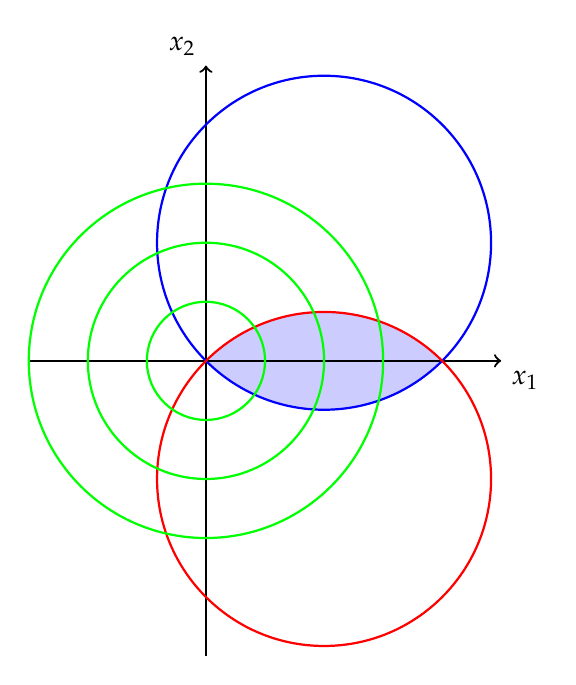
\begin{tikzpicture}[scale=1.5]
\begin{scope}
\clip (1,1) circle (1.414);
\fill[blue!20] (1,-1) circle (1.414);
\end{scope}
\draw[thick,->] (-1.5,0) -- (2.5,0) node[anchor=north west] {$x_1$};
\draw[thick,->] (0,-2.5) -- (0,2.5) node[anchor=south east] {$x_2$};
\draw[thick,blue] (1,1) circle (1.414);
\draw[thick,red] (1,-1) circle (1.414);
\draw[thick,green] (0,0) circle (0.5);
\draw[thick,green] (0,0) circle (1);
\draw[thick,green] (0,0) circle (1.5);
\end{tikzpicture}
\caption{Feasible region and level sets of the objective function}
\end{figure}

\[
x^\star=(0,0)
\]

with optimal value

\[
p^\star=0.
\]

\item[(b)]

The problem is convex because

\begin{itemize}
\item the objective $x_1^2+x_2^2$ is convex,
\item the constraint functions
\[
g_1(x)=(x_1-1)^2+(x_2-1)^2-2
\]
and
\[
g_2(x)=(x_1-1)^2+(x_2+1)^2-2
\]
are convex.
\end{itemize}

To verify strong duality we check Slater's condition. Consider the point $x=(1,0)$:

\[
(1-1)^2+(0-1)^2=1<2
\]

\[
(1-1)^2+(0+1)^2=1<2
\]

Thus a strictly feasible point exists, so Slater's condition holds. Therefore strong duality holds.

\item[(c)]

Define

\[
g_1(x)=(x_1-1)^2+(x_2-1)^2-2,
\quad
g_2(x)=(x_1-1)^2+(x_2+1)^2-2.
\]

The Lagrangian is

\[
L(x,\lambda_1,\lambda_2)
=
x_1^2+x_2^2
+
\lambda_1 g_1(x)
+
\lambda_2 g_2(x).
\]

The KKT conditions are

\textit{Primal feasibility}
\[
g_1(x^\star)\le0,\quad g_2(x^\star)\le0
\]

\textit{Dual feasibility}
\[
\lambda_1^\star\ge0,\quad \lambda_2^\star\ge0
\]

\textit{Complementary slackness}
\[
\lambda_1^\star g_1(x^\star)=0,
\quad
\lambda_2^\star g_2(x^\star)=0
\]

\textit{Stationarity}
\[
\nabla f(x^\star)
+
\lambda_1^\star \nabla g_1(x^\star)
+
\lambda_2^\star \nabla g_2(x^\star)
=0.
\]

Compute gradients:

\[
\nabla f(x)=
\begin{bmatrix}
2x_1\\
2x_2
\end{bmatrix},
\quad
\nabla g_1(x)=
\begin{bmatrix}
2(x_1-1)\\
2(x_2-1)
\end{bmatrix},
\quad
\nabla g_2(x)=
\begin{bmatrix}
2(x_1-1)\\
2(x_2+1)
\end{bmatrix}.
\]

At $x^\star=(0,0)$:

\[
\nabla f(x^\star)=
\begin{bmatrix}
0\\
0
\end{bmatrix},
\quad
\nabla g_1(x^\star)=
\begin{bmatrix}
-2\\
-2
\end{bmatrix},
\quad
\nabla g_2(x^\star)=
\begin{bmatrix}
-2\\
2
\end{bmatrix}.
\]

Stationarity gives

\[
\lambda_1^\star
\begin{bmatrix}
-2\\
-2
\end{bmatrix}
+
\lambda_2^\star
\begin{bmatrix}
-2\\
2
\end{bmatrix}
=
\begin{bmatrix}
0\\
0
\end{bmatrix}.
\]

Thus

\[
\lambda_1^\star=\lambda_2^\star=0.
\]

These satisfy all KKT conditions, confirming that $x^\star=(0,0)$ is optimal.
\end{enumerate}


%----------------------------------------------------------------------------------------
\newpage
\section*{Problem 3. Strong Duality but No KKT}

In this question, we will see an example of a problem where strong duality holds but the KKT conditions don’t hold.

Consider the following problem:

\[
p^\star = \min_{x_1,x_2 \in \mathbb{R}} x_1^2 + x_2^2
\tag{14}
\]

\[
\text{s.t. } (x_1 - 1)^2 + (x_2 - 1)^2 \le 1
\tag{15}
\]

\[
(x_1 - 1)^2 + (x_2 + 1)^2 \le 1
\tag{16}
\]

(a) Sketch the feasible set.
Find the optimal solution \(x^\star\).

(b) Write the KKT conditions and solve them.

(c) Formulate and solve the Lagrange dual problem.
Does strong duality hold?

\subsection*{Answer}

\begin{enumerate}

\item[(a)]

The constraints define two disks

\[
(x_1-1)^2+(x_2-1)^2 \le 1
\]


\[
(x_1-1)^2+(x_2+1)^2 \le 1
\]

Thus the two disks touch at exactly one point:

\[
x^\star=(1,0).
\]

Since this is the only feasible point, it is automatically optimal. The optimal value is

\[
p^\star = 1^2+0^2 = 1.
\]

\item[(b)]

Define

\[
g_1(x)=(x_1-1)^2+(x_2-1)^2-1,
\qquad
g_2(x)=(x_1-1)^2+(x_2+1)^2-1.
\]

The KKT conditions are

\begin{itemize}
\item Primal feasibility: $g_1(x^\star)\le0$, $g_2(x^\star)\le0$
\item Dual feasibility: $\lambda_1,\lambda_2\ge0$
\item Complementary slackness: $\lambda_1 g_1(x^\star)=0$, $\lambda_2 g_2(x^\star)=0$
\item Stationarity:
\[
\nabla f(x^\star)+\lambda_1\nabla g_1(x^\star)+\lambda_2\nabla g_2(x^\star)=0.
\]
\end{itemize}

Compute gradients:

\[
\nabla f(x)=
\begin{bmatrix}
2x_1\\
2x_2
\end{bmatrix},
\quad
\nabla g_1(x)=
\begin{bmatrix}
2(x_1-1)\\
2(x_2-1)
\end{bmatrix},
\quad
\nabla g_2(x)=
\begin{bmatrix}
2(x_1-1)\\
2(x_2+1)
\end{bmatrix}.
\]

At \(x^\star=(1,0)\):

\[
\nabla f(x^\star)=
\begin{bmatrix}
2\\
0
\end{bmatrix},
\quad
\nabla g_1(x^\star)=
\begin{bmatrix}
0\\
-2
\end{bmatrix},
\quad
\nabla g_2(x^\star)=
\begin{bmatrix}
0\\
2
\end{bmatrix}.
\]

Stationarity becomes

\[
\begin{bmatrix}
2\\
0
\end{bmatrix}
+
\lambda_1
\begin{bmatrix}
0\\
-2
\end{bmatrix}
+
\lambda_2
\begin{bmatrix}
0\\
2
\end{bmatrix}
=
\begin{bmatrix}
0\\
0
\end{bmatrix}.
\]

From the first coordinate,

\[
2=0,
\]

which is impossible. Therefore no multipliers $\lambda_1,\lambda_2$ satisfy the KKT conditions.

\item[(c)]

The Lagrangian is

\[
L(x,\lambda_1,\lambda_2)
=
x_1^2+x_2^2
+\lambda_1\big((x_1-1)^2+(x_2-1)^2-1\big)
+\lambda_2\big((x_1-1)^2+(x_2+1)^2-1\big).
\]

Minimizing over $x$ gives

\[
x_1=\frac{\lambda_1+\lambda_2}{\lambda_1+\lambda_2+1},
\qquad
x_2=\frac{\lambda_1-\lambda_2}{\lambda_1+\lambda_2+1}.
\]

Substituting into the Lagrangian yields the dual function

\[
g(\lambda_1,\lambda_2)
=
\frac{-\lambda_1^2+2\lambda_1\lambda_2-\lambda_2^2+\lambda_1+\lambda_2}
{\lambda_1+\lambda_2+1}
= \frac{(\lambda_1-\lambda_2)^2+\lambda_1+\lambda_2}{\lambda_1+\lambda_2+1}
\]

The dual problem is

\[
\max_{\lambda_1,\lambda_2\ge0} g(\lambda_1,\lambda_2).
\]

Setting $\lambda_1=\lambda_2=t$ gives

\[
g(t,t)=\frac{2t}{2t+1}.
\]

As $t\to\infty$,

\[
g(t,t)\to1.
\]

Thus the dual optimal value is

\[
d^\star=1.
\]

Since
$ d^\star=p^\star=1, $
strong duality holds, even though the KKT conditions do not hold.

\end{enumerate}


%----------------------------------------------------------------------------------------
\newpage
\section*{Problem 4. Does Strong Duality Hold?}

Consider

\[
\min_{(x,y)\in D} e^{-x}
\tag{17}
\]

\[
\text{s.t. } \frac{x^2}{y} \le 0
\tag{18}
\]

where \(D = \{(x,y) \mid y > 0\}\).

(a) Prove the problem is convex.
Find the optimal value.

HINT: To prove the constraint function is convex, you will have to prove it is convex with respect to the vector \([x\;y]^\top\).
Consider computing the Hessian of the constraint function, its determinant and trace, and show that it is PSD by analyzing signs of its eigenvalues.

(b) Next, we will proceed to find an optimal solution and an optimal value for the dual problem.
The Lagrangian dual function \(g(\lambda)\) can be written as

\[
g(\lambda) = \inf_{(x,y)\in D} e^{-x} + \lambda \frac{x^2}{y}
\tag{19}
\]

Explain why \(g(\lambda)\) is lower bounded by 0 for \(\lambda \ge 0\).

NOTE: Here we are not dualizing the constraint \(y > 0\) that is in the definition of \(D\) — this is only dualizing the other constraint.

(c) Show that \(g(\lambda) = 0\) for \(\lambda \ge 0\).

HINT: To show that the infimum in (19) is 0, we want to show there exist \((x,y)\) such that both \(e^{-x}\) and \(\lambda x^2/y\) can get arbitrarily close to 0.

HINT: Consider a sequence \(\{x_k\}\) going to \(+\infty\) and a sequence \(\{y_k\}\) also going to \(+\infty\) such that

\[
\lim_{k\to\infty} \frac{x_k^2}{y_k} = 0.
\]

Simply put, we want to drive \(x\) to infinity in order to drive \(e^{-x}\) to 0,
while having \(y\) grow faster than \(x^2\), so that the second term also goes to 0.

(d) Now, write the dual problem and find an optimal solution \(\lambda^\star\) and an optimal value \(d^\star\) for the dual problem using the results above.
What is the duality gap?

(e) Does Slater’s Condition hold for this problem?
Does Strong Duality hold?

\subsection*{Answer}

\begin{enumerate}

\item[(a)]

The objective function \(f_0(x,y)=e^{-x}\) is convex since
\[
\frac{d^2}{dx^2}e^{-x}=e^{-x}>0.
\]

The constraint function is
\[
f(x,y)=\frac{x^2}{y}, \qquad y>0.
\]

Compute the gradient
\[
\nabla f(x,y)=
\begin{bmatrix}
\frac{2x}{y}\\[4pt]
-\frac{x^2}{y^2}
\end{bmatrix}.
\]

The Hessian is
\[
\nabla^2 f(x,y)=
\begin{bmatrix}
\frac{2}{y} & -\frac{2x}{y^2}\\[6pt]
-\frac{2x}{y^2} & \frac{2x^2}{y^3}
\end{bmatrix}.
\]

Compute the determinant

\[
\det(\nabla^2 f)
=
\frac{2}{y}\cdot\frac{2x^2}{y^3}
-
\left(-\frac{2x}{y^2}\right)^2
=
\frac{4x^2}{y^4}-\frac{4x^2}{y^4}
=0.
\]

The trace is

\[
\text{tr}(\nabla^2 f)
=
\frac{2}{y}+\frac{2x^2}{y^3}>0
\qquad (y>0).
\]

Since the determinant is nonnegative and the trace is positive,
both eigenvalues are nonnegative, so the Hessian is PSD.
Thus \(x^2/y\) is convex in \((x,y)\).

Hence the problem is a convex optimization problem.

The constraint

\[
\frac{x^2}{y}\le0
\]

with \(y>0\) implies

\[
x^2\le0,
\]

so

\[
x=0.
\]

Thus the feasible set is

\[
\{(0,y)\mid y>0\}.
\]

The objective becomes

\[
e^{-0}=1.
\]

Hence the optimal value is

\[
p^\star=1.
\]

\item[(b)]

The dual function is

\[
g(\lambda)=\inf_{(x,y)\in D}\left(e^{-x}+\lambda\frac{x^2}{y}\right).
\]

For \(\lambda\ge0\),

\[
e^{-x}\ge0, \qquad \lambda\frac{x^2}{y}\ge0
\]

because \(y>0\).

Thus

\[
e^{-x}+\lambda\frac{x^2}{y}\ge0
\]

for all \((x,y)\in D\), which implies

\[
g(\lambda)\ge0.
\]

\item[(c)]

Consider sequences \(x_k\to\infty\) and \(y_k\to\infty\) such that

\[
\frac{x_k^2}{y_k}\to0.
\]

For example, take

\[
y_k=x_k^3.
\]

Then

\[
\frac{x_k^2}{y_k}=\frac{x_k^2}{x_k^3}=\frac{1}{x_k}\to0.
\]

As \(x_k\to\infty\),

\[
e^{-x_k}\to0.
\]

Thus both terms in

\[
e^{-x_k}+\lambda\frac{x_k^2}{y_k}
\]

approach 0, so the infimum is 0. Therefore

\[
g(\lambda)=0
\qquad \text{for all } \lambda\ge0.
\]

\item[(d)]

The dual problem is

\[
\max_{\lambda\ge0} g(\lambda).
\]

Since \(g(\lambda)=0\) for all \(\lambda\ge0\),

\[
d^\star=0.
\]

Any \(\lambda^\star\ge0\) is optimal.

The primal optimal value is

\[
p^\star=1.
\]

Thus the duality gap is

\[
p^\star-d^\star=1.
\]

\item[(e)]

Slater’s condition requires a strictly feasible point satisfying

\[
\frac{x^2}{y}<0.
\]

Since \(x^2\ge0\) and \(y>0\),

\[
\frac{x^2}{y}\ge0
\]

for all feasible points, so the inequality cannot be strict.

Thus Slater’s condition does not hold.

Since

\[
p^\star\ne d^\star,
\]

strong duality does not hold.

\end{enumerate}


%----------------------------------------------------------------------------------------

\newpage
\section*{Problem 5. Water Filling}

Consider the following problem:

\[
\text{minimize } -\sum_{i=1}^{n} \log(\alpha_i + x_i)
\tag{20}
\]

\[
\text{subject to } x \ge 0,\quad \mathbf{1}^\top x = c
\tag{21}
\]

where \(\alpha_i > 0\) for each \(i = 1,\ldots,n\).

This problem arises in information theory, in allocating power to a set of \(n\) communication channels.

The variable \(x_i\) represents the transmitter power allocated to the \(i\)th channel,
and \(\log(\alpha_i + x_i)\) gives the capacity or communication rate of the channel,
so the problem is to allocate a total power of \(c\) to the channels,
in order to maximize the total communication rate.

(a) Verify that this is a convex optimization problem with differentiable objective and constraint functions.
Find the domain \(D\) of the objective function \(-\sum_{i=1}^n \log(\alpha_i + x_i)\) where it is well defined.

(b) Let \(\lambda \in \mathbb{R}^n\) and \(\nu \in \mathbb{R}\) be the dual variables corresponding to the constraints \(x_i \ge 0\) and \(\mathbf{1}^\top x = c\).
Write a Lagrangian for the optimization problem based on these dual variables.

(c) Write the KKT conditions for the problem.

(d) Since our problem is a convex optimization problem with differentiable objective and constraint functions,
the KKT conditions provide sufficient conditions for optimality.

Hence, we know that if we can find \(x^\star\) and \((\lambda^\star, \nu^\star)\) that satisfy the KKT conditions,
then \(x^\star\) will be a primal optimal point and \((\lambda^\star, \nu^\star)\) will be dual optimal.

We therefore attempt to find solutions for the KKT conditions.

As a first step, show how to simplify the KKT conditions so that they are expressed in terms of only \(x^\star\) and \(\nu^\star\),
i.e. show how \(\lambda^\star\) can be eliminated from these conditions.

(e) Solve for \(x_i^\star\) in terms of \(\nu^\star\).

\subsection*{Answer}

\begin{enumerate}

\item[(a)]

The objective function is
\[
f(x)=-\sum_{i=1}^n \log(\alpha_i+x_i).
\]

Since $\log(\cdot)$ is concave on $(0,\infty)$, $-\log(\cdot)$ is convex.
Because $\alpha_i+x_i$ is affine in $x_i$, each term $-\log(\alpha_i+x_i)$ is convex.
A sum of convex functions is convex, so the objective is convex.

The constraints are
\[
x_i\ge0, \qquad \mathbf{1}^\top x=c.
\]

The inequality constraints are affine and the equality constraint is affine,
so the feasible set is convex.

Therefore the problem is a convex optimization problem with differentiable
objective and constraint functions.

The logarithm requires
\[
\alpha_i+x_i>0.
\]

Thus the domain of the objective function is

\[
D=\{x\in\mathbb{R}^n \mid \alpha_i+x_i>0,\; i=1,\ldots,n\}.
\]

Since $\alpha_i>0$ and $x_i\ge0$, every feasible point lies in this domain.

\item[(b)]

Let $\lambda\in\mathbb{R}^n$ be the dual variables for the constraints
$x_i\ge0$ and $\nu\in\mathbb{R}$ be the dual variable for
$\mathbf{1}^\top x=c$.

Writing the inequality constraints as $-x_i\le0$, the Lagrangian is

\[
L(x,\lambda,\nu)
=
-\sum_{i=1}^n \log(\alpha_i+x_i)
-\sum_{i=1}^n \lambda_i x_i
+\nu(\mathbf{1}^\top x-c).
\]

\item[(c)]

The KKT conditions are:

\textit{Primal feasibility}
\[
x_i^\star \ge 0, \qquad \mathbf{1}^\top x^\star=c.
\]

\textit{Dual feasibility}
\[
\lambda_i^\star \ge 0.
\]

\textit{Complementary slackness}
\[
\lambda_i^\star x_i^\star=0, \qquad i=1,\ldots,n.
\]

\textit{Stationarity}

\[
\nabla_x L(x^\star,\lambda^\star,\nu^\star)=0.
\]

Compute the gradient:

\[
\frac{\partial L}{\partial x_i}
=
-\frac{1}{\alpha_i+x_i}
-\lambda_i
+\nu.
\]

Thus stationarity gives

\[
-\frac{1}{\alpha_i+x_i^\star}-\lambda_i^\star+\nu^\star=0,
\qquad i=1,\ldots,n.
\]

\item[(d)]

From the stationarity condition,

\[
\lambda_i^\star
=
\nu^\star-\frac{1}{\alpha_i+x_i^\star}.
\]

Substitute this expression into the dual feasibility condition
$\lambda_i^\star\ge0$:

\[
\nu^\star-\frac{1}{\alpha_i+x_i^\star}\ge0.
\]

Substitute it into complementary slackness:

\[
\left(\nu^\star-\frac{1}{\alpha_i+x_i^\star}\right)x_i^\star=0.
\]

Thus the KKT conditions can be written only in terms of
$x^\star$ and $\nu^\star$ as

\[
x_i^\star\ge0,
\]

\[
\nu^\star-\frac{1}{\alpha_i+x_i^\star}\ge0,
\]

\[
\left(\nu^\star-\frac{1}{\alpha_i+x_i^\star}\right)x_i^\star=0,
\]

\[
\sum_{i=1}^n x_i^\star=c.
\]

\item[(e)]

From complementary slackness,

\[
\left(\nu^\star-\frac{1}{\alpha_i+x_i^\star}\right)x_i^\star=0.
\]

If $x_i^\star>0$, then

\[
\nu^\star=\frac{1}{\alpha_i+x_i^\star}.
\]

Solving for $x_i^\star$ gives

\[
x_i^\star=\frac{1}{\nu^\star}-\alpha_i.
\]

Combining with the constraint $x_i^\star\ge0$,

\[
x_i^\star=\max\left(0,\frac{1}{\nu^\star}-\alpha_i\right).
\]

This is the water-filling solution.
\end{enumerate}


%----------------------------------------------------------------------------------------

\section*{Problem 6. Homework Process}

With whom did you work on this homework?
List the names and SIDs of your group members.

NOTE: If you didn’t work with anyone, you can put “none” as your answer.

\subsection*{Answer}

none
\end{document}
